\chapter{Análisis y diseño de la propuesta de solución}
\label{chap:chapter2}

El presente capítulo constituye el núcleo de la fase de análisis y diseño de la investigación, traduciendo
los fundamentos teóricos establecidos en el capítulo anterior en una propuesta técnica concreta y viable.
Partiendo del diagnóstico de la problemática y del estudio de sistemas homólogos, se procede a definir de
manera formal y estructurada la solución de software que dará respuesta al objetivo general de la investigación.

El capítulo se inicia con la propuesta de solución, que describe a alto nivel el sistema a desarrollar. 
A continuación, se realiza un levantamiento detallado de requisitos, clasificados en funcionales y no
funcionales, para precisar el comportamiento y las cualidades del sistema. Estas especificaciones se refinan
a través de \ac{HU}, las cuales, junto con su estimación de esfuerzo, sirven de base para el desarrollo del plan de
iteraciones que guiará la implementación. Posteriormente, el diseño orientado a objetos se plasma mediante
tarjetas \ac{CRC}, sentando las bases para la definición de la arquitectura de software basada en el patrón 
\textbf{ARQUITECTURA}. Finalmente, se especifican los \ac{GRASP} y los patrones de diseño \ac{GoF},  
que se aplicarán para resolver problemas comunes en el desarrollo de software y otros ámbitos referentes 
al diseño.

\section{Descripcion de la propuesta de solución}

En función de dar cumplimiento al objetivo planteado y ajustándose a las necesidades presentes,
se propone desarrollar un servicio \textit{backend} que, basado en los principios de \ac{SPLE}
y la técnica de modelado \ac{FM}, permita a los profesionales de la educación representar y 
gestionar la variabilidad curricular de forma sistemática utilizando \ac{UVL} como lenguaje de 
modelado u operando directamente sobre la representación gráfica. Esta solución permitirá representar 
formalmente planes de estudio, definir variabilidad entre módulos, establecer dependencias,
restricciones y rutas formativas alternativas, así como derivar configuraciones 
válidas que representen itinerarios personalizados. En esencia,
el sistema habilita una ingeniería curricular basada en la lógica \ac{SPLE},
donde los planes de estudio se conciben como familias de productos y
cada configuración curricular corresponde a un producto derivado.

El servicio abordará todas las fases necesarias para este proceso: 
diseño del modelo curricular (equivalente al análisis de dominio),
definición de restricciones y cardinalidades (gestión de variabilidad), validación 
automatizada de configuraciones (ensamblaje de productos) y
versionamiento del modelo (gestión de activos). Para ello se implementará 
un motor central que permita representar jerarquías de características, 
aplicar reglas transversales, procesar requerimientos, exclusiones
e implicaciones, y generar configuraciones consistentes, detectando violaciones 
y proponiendo alternativas.

El sistema incorporará funcionalidades que responden directamente
a los retos del dominio educativo: evitar inconsistencias curriculares, detectar 
prerrequisitos no satisfechos, prevenir combinaciones inviables,
explorar rutas posibles, permitir adaptaciones por niveles, perfiles o competencias 
y almacenar \textit{snapshots} versionados que faciliten la evolución
del plan de estudios sin invalidar configuraciones previas. Este enfoque
no se limita a documentar un currículo, sino que lo convierte en un modelo 
computable y verificable, habilitando su reutilización y variación controlada.




% ======================================
% 		--- PLANTILLA ---
% ======================================

\section{Sección de prueba}
Escribir aquí el capítulo 2. Prueba de glosario  \gls{Engine}. A continuación un ejemplo de enlace al anexo \hyperlink{bloque.1}{Bloque Corona}. Este es un ejemplo de matriz con bordes numerados \citep{Mathew2010}.

\newcommand{\colorentrygreen}[1]{\multicolumn{1}{c}{\cellcolor{green!20} #1}}
\newcommand{\colorentryred}[1]{\multicolumn{1}{c}{\cellcolor{red!20} #1}}

\begin{align*}
	\kbordermatrix
	{
		Padre&1&2&3&4\\
		1&\colorentrygreen{0}&\colorentrygreen{1}&\colorentrygreen{0}&\colorentrygreen{0}\\
		2&0&0&0&1\\
		3&\colorentrygreen{1}&\colorentrygreen{0}&\colorentrygreen{0}&\colorentrygreen{0}\\
		4&0&0&1&0
	}
	\begin{array}{l}
		\rightarrow \mbox{Seleccionada aleatoriamente}\\
		\quad\\
		\rightarrow \mbox{Seleccionada aleatoriamente}\\
		\quad\\
	\end{array}
	\qquad
	\kbordermatrix
	{
		Madre&1&2&3&4\\
		1&1&0&0&0\\
		2&0&1&0&0\\
		3&\colorentryred{0}&\colorentryred{0}&\colorentryred{1}&\colorentryred{0}\\
		4&\colorentryred{0}&\colorentryred{0}&\colorentryred{0}&\colorentryred{1}
	}
\end{align*}
\begin{align}
\stackrel{\quad Hijo}
{
	\kbordermatrix
	{
		 &1&2&3&4\\
		1&\colorentrygreen{0}&\colorentrygreen{1}&\colorentrygreen{0}&\colorentrygreen{0}\\
		2&\colorentryred{0}&\colorentryred{0}&\colorentryred{1}&\colorentryred{0}\\
		3&\colorentrygreen{1}&\colorentrygreen{0}&\colorentrygreen{0}&\colorentrygreen{0}\\
		4&\colorentryred{0}&\colorentryred{0}&\colorentryred{0}&\colorentryred{1}
	}
}
\end{align}

\lipsum[1-2]
\hlblock{Este es un ejemplo de cita \citep{Mathew2010}
Esta es una prueba de cómo se escribe un pseudocódigo en \LaTeX.}
\begin{algorithm}[!h]
\caption{Estrategia de BellmanKalaba}\label{alg:algorithtest}
  \begin{algorithmic}[1]
\Procedure {BellmanKalaba}{$G$, $u$, $l$, $p$}
  \ForAll {$v \in V(G)$}
    \State $l(v) \leftarrow \infty$
  \EndFor
  \State $l(u) \leftarrow 0$
  \Repeat
    \For {$i \leftarrow 1, n$}
      \State $min \leftarrow l(v_i)$
      \For {$j \leftarrow 1, n$}
        \If {$min > e(v_i, v_j) + l(v_j)$}
          \State $min \leftarrow e(v_i, v_j) + l(v_j)$
          \State $p(i) \leftarrow v_j$
        \EndIf
      \EndFor
    \State $l'(i) \leftarrow min$
    \EndFor
  \State $changed \leftarrow l \not= l'$
  \State $l \leftarrow l'$
  \Until{$\neg changed$}
\EndProcedure
\end{algorithmic}
\end{algorithm}

\section{Ejemplos de código fuente}
\lipsum[2-4]
Este es un ejemplo de cita \citep{Mathew2010}
\singlespacing
\loadlanguage{C++}
\lstinputlisting[tabsize=3, breaklines, frame=lines, firstline=1, lastline=14, caption=Búsqueda de máximo]{Anexos/code.cpp}

\loadlanguage{Java}
\lstinputlisting[tabsize=3, breaklines, frame=lines, firstline=17, lastline=27, caption=Ejemplo de código en Java]{Anexos/code.cpp}

\loadlanguage{PHP}
\lstset{emph=[3]{join, condition, idtarea, nombre, descripcion, idinstructora, fecha}} % attributes
\lstinputlisting[tabsize=3, breaklines, frame=lines, firstline=29, lastline=60, caption=Ejemplo de código en PHP]{Anexos/code.cpp}

\loadlanguage{PHP}
\lstinputlisting[tabsize=3, breaklines, frame=lines, firstline=147, caption=Ejemplo de código en PHP]{Anexos/code.cpp}

\loadlanguage{Python}
\lstinputlisting[tabsize=3, breaklines, frame=lines, firstline=62, lastline=67, caption=Ejemplo de código en Python]{Anexos/code.cpp}

\lstinputlisting[style=htmlcssjs, tabsize=3, breaklines, frame=lines, firstline=69, lastline=87, caption=Ejemplo de código en htmlcssjs]{Anexos/code.cpp}

\lstinputlisting[style=htmlcssjs, tabsize=3, breaklines, frame=lines, firstline=89, lastline=146, caption=Ejemplo de código en htmlcssjs]{Anexos/code.cpp}



\chapter{Ejemplo de tabla grande}
   \section{Tabla aleatoria}
   
   
  
   \begin{longtable}[c]{|l|l|l|}
	   \captionsetup{margin=1.15\leftmargin}
	   \caption{Feasible triples for highly variable Grid, MLMMH.}
	   \label{grid_mlmmh} \\[2ex]
	   
	   \hline \multicolumn{1}{|c|}{\textbf{Time (s)}} & \multicolumn{1}{c|}{\textbf{Triple chosen}} & \multicolumn{1}{c|}{\textbf{Other feasible triples}} \\ \hline 
	   \endfirsthead
	   
	   \caption{continued from previous page} \\
	   \hline \multicolumn{1}{|c|}{\textbf{Time (s)}} &
	   \multicolumn{1}{c|}{\textbf{Triple chosen}} &
	   \multicolumn{1}{c|}{\textbf{Other feasible triples}} \\ \hline 
	   \endhead
	   
	   \hline \multicolumn{3}{|r|}{{Continued on next page}} \\ \hline
	   \endfoot
	   
	   \hline
	   \endlastfoot
	   
	   0 & (1, 11, 13725) & (1, 12, 10980), (1, 13, 8235), (2, 2, 0), (3, 1, 0) \\ \cline{2-3}
	   2745 & (1, 12, 10980) & (1, 13, 8235), (2, 2, 0), (2, 3, 0), (3, 1, 0) \\
	   5490 & (1, 12, 13725) & (2, 2, 2745), (2, 3, 0), (3, 1, 0) \\
	   8235 & (1, 12, 16470) & (1, 13, 13725), (2, 2, 2745), (2, 3, 0), (3, 1, 0) \\
	   10980 & (1, 12, 16470) & (1, 13, 13725), (2, 2, 2745), (2, 3, 0), (3, 1, 0) \\
	   13725 & (1, 12, 16470) & (1, 13, 13725), (2, 2, 2745), (2, 3, 0), (3, 1, 0) \\
	   16470 & (1, 13, 16470) & (2, 2, 2745), (2, 3, 0), (3, 1, 0) \\
	   19215 & (1, 12, 16470) & (1, 13, 13725), (2, 2, 2745), (2, 3, 0), (3, 1, 0) \\
	   21960 & (1, 12, 16470) & (1, 13, 13725), (2, 2, 2745), (2, 3, 0), (3, 1, 0) \\
	   24705 & (1, 12, 16470) & (1, 13, 13725), (2, 2, 2745), (2, 3, 0), (3, 1, 0) \\
	   27450 & (1, 12, 16470) & (1, 13, 13725), (2, 2, 2745), (2, 3, 0), (3, 1, 0) \\
	   30195 & (2, 2, 2745) & (2, 3, 0), (3, 1, 0) \\
	   32940 & (1, 13, 16470) & (2, 2, 2745), (2, 3, 0), (3, 1, 0) \\
	   35685 & (1, 13, 13725) & (2, 2, 2745), (2, 3, 0), (3, 1, 0) \\
	   38430 & (1, 13, 10980) & (2, 2, 2745), (2, 3, 0), (3, 1, 0) \\
	   41175 & (1, 12, 13725) & (1, 13, 10980), (2, 2, 2745), (2, 3, 0), (3, 1, 0) \\
	   43920 & (1, 13, 10980) & (2, 2, 2745), (2, 3, 0), (3, 1, 0) \\
	   46665 & (2, 2, 2745) & (2, 3, 0), (3, 1, 0) \\
	   49410 & (2, 2, 2745) & (2, 3, 0), (3, 1, 0) \\
	   52155 & (1, 12, 16470) & (1, 13, 13725), (2, 2, 2745), (2, 3, 0), (3, 1, 0) \\
	   54900 & (1, 13, 13725) & (2, 2, 2745), (2, 3, 0), (3, 1, 0) \\
	   57645 & (1, 13, 13725) & (2, 2, 2745), (2, 3, 0), (3, 1, 0) \\
	   60390 & (1, 12, 13725) & (2, 2, 2745), (2, 3, 0), (3, 1, 0) \\
	   63135 & (1, 13, 16470) & (2, 2, 2745), (2, 3, 0), (3, 1, 0) \\
	   65880 & (1, 13, 16470) & (2, 2, 2745), (2, 3, 0), (3, 1, 0) \\
	   68625 & (2, 2, 2745) & (2, 3, 0), (3, 1, 0) \\
	   71370 & (1, 13, 13725) & (2, 2, 2745), (2, 3, 0), (3, 1, 0) \\
	   74115 & (1, 12, 13725) & (2, 2, 2745), (2, 3, 0), (3, 1, 0) \\
	   76860 & (1, 13, 13725) & (2, 2, 2745), (2, 3, 0), (3, 1, 0) \\
	   79605 & (1, 13, 13725) & (2, 2, 2745), (2, 3, 0), (3, 1, 0) \\
	   82350 & (1, 12, 13725) & (2, 2, 2745), (2, 3, 0), (3, 1, 0) \\
	   85095 & (1, 12, 13725) & (1, 13, 10980), (2, 2, 2745), (2, 3, 0), (3, 1, 0) \\
	   87840 & (1, 13, 16470) & (2, 2, 2745), (2, 3, 0), (3, 1, 0) \\
	   90585 & (1, 13, 16470) & (2, 2, 2745), (2, 3, 0), (3, 1, 0) \\
	   93330 & (1, 13, 13725) & (2, 2, 2745), (2, 3, 0), (3, 1, 0) \\
	   96075 & (1, 13, 16470) & (2, 2, 2745), (2, 3, 0), (3, 1, 0) \\
	   98820 & (1, 13, 16470) & (2, 2, 2745), (2, 3, 0), (3, 1, 0) \\
	   101565 & (1, 13, 13725) & (2, 2, 2745), (2, 3, 0), (3, 1, 0) \\
	   104310 & (1, 13, 16470) & (2, 2, 2745), (2, 3, 0), (3, 1, 0) \\
	   107055 & (1, 13, 13725) & (2, 2, 2745), (2, 3, 0), (3, 1, 0) \\
	   109800 & (1, 13, 13725) & (2, 2, 2745), (2, 3, 0), (3, 1, 0) \\
	   112545 & (1, 12, 16470) & (1, 13, 13725), (2, 2, 2745), (2, 3, 0), (3, 1, 0) \\
	   115290 & (1, 13, 16470) & (2, 2, 2745), (2, 3, 0), (3, 1, 0) \\
	   118035 & (1, 13, 13725) & (2, 2, 2745), (2, 3, 0), (3, 1, 0) \\
	   120780 & (1, 13, 16470) & (2, 2, 2745), (2, 3, 0), (3, 1, 0) \\
	   123525 & (1, 13, 13725) & (2, 2, 2745), (2, 3, 0), (3, 1, 0) \\
	   126270 & (1, 12, 16470) & (1, 13, 13725), (2, 2, 2745), (2, 3, 0), (3, 1, 0) \\
	   129015 & (2, 2, 2745) & (2, 3, 0), (3, 1, 0) \\
	   131760 & (2, 2, 2745) & (2, 3, 0), (3, 1, 0) \\
	\end{longtable}

\section{Tablas de ingeniería}

\begin{userstory}[tb:prueba]
	\storyname{Cargar archivo}
	\storyuser{Especialista}
	\storyiter{1}
	\storypriority{Alta}
	\storyrisk{Bajo}
	\storypoints{0.8}
	\storyprogrammer{Ernesto Gil Capote}
	\storydescription{
	Permite cargar los datos de los casos de estudio a utilizar en el módulo con el objetivo de determinar secuencias factibles. Estos están almacenados en archivos con extensión .asp. La estructura está compuesta por los parámetros de entrada de la aplicación para cada caso de estudio tales como: dimensión, nombre de la estructura mecánica, cantidad de piezas, la MD correspondiente y el vector de herramientas en caso de que lo posea.
	\begin{itemize}
	\item rojo
	\item blanco
	\end{itemize}
	}
	\storyobservation{En caso de que el usuario no cargue un archivo, el sistema debe mostrar un mensaje de alerta con dicha explicación. Si se introduce un archivo que contiene caracteres no válidos o falta alguno de los elementos necesarios para la ejecución del módulo, este debe lanzar la excepción correspondiente.En caso de que el usuario no cargue un archivo, el sistema debe mostrar un mensaje de alerta con dicha explicación. Si se introduce un archivo que contiene caracteres no válidos o falta alguno de los elementos necesarios para la ejecución del módulo, este debe lanzar la excepción correspondiente.}
	%\storyinterface{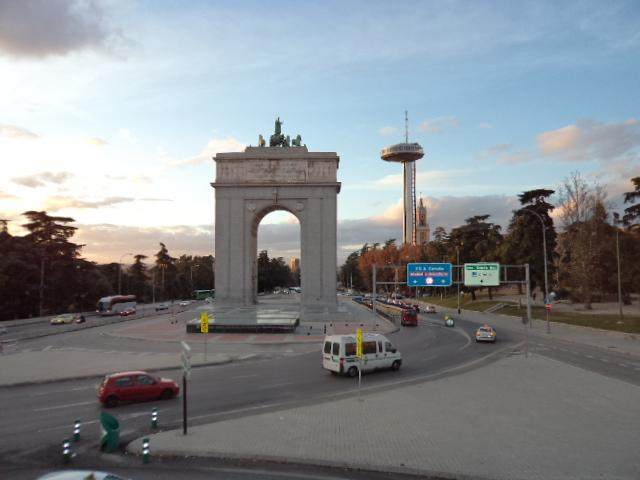
\includegraphics[scale=0.5]{Images/DSC00461}}
\end{userstory}

Esta es referencia a una tabla de historia de usuario \ref{tb:prueba}

\begin{crccard}[tablacrc3]
\crcclass{AlgoritmoGenetico}
\crcresp
{
	\begin{itemize}
	\item Crear el conjunto de genes necesarios para la creación de un individuo
	\item Realizar el proceso de mutación y recombinación
	\item Crear el conjunto de genes necesarios para la creación de un individuo
	\item Realizar el proceso de mutación y recombinación
	\end{itemize}
}
\crccolab
{
	Población\\
	OperadorProbabilidad\\
	OperadorParejas\\
	OperadorReproducion\\
	Población
}
\end{crccard}

\begin{crccard}[tablacrc2]
\crcclass{AlgoritmoGenetico}
\crcresp
{
	\begin{itemize}
	\item Crear el conjunto de genes necesarios para la creación de un individuo
	\item Realizar el proceso de mutación y recombinación
	\item Crear el conjunto de genes necesarios para la creación de un individuo
	\item Realizar el proceso de mutación y recombinación
	\end{itemize}
}
\crccolab
{
	Población\\
	OperadorProbabilidad\\
	OperadorParejas\\
	OperadorReproducion\\
	Población
}
\end{crccard}


\begin{effortestimation}[tb:est1]
	\addentry[2]{Graficar secuencias de ensamble}{0.3} 
	\addentry[2]{Graficar secuencias de ensamble}{0.3} 
	\addentry[2]{Graficar secuencias de ensamble}{0.3} 
	\addentry[2]{Graficar secuencias de ensamble}{0.2}
	\addentry[2]{Graficar secuencias de ensamble}{0.2} 
	\addentry[4]{Graficar secuencias de ensamble}{0.1} 
	\addentry[4]{Graficar ensamble}{0.1} 
	\addentry[3]{Determinar Secuencia de Ensamble}{0.5} 
	\addentry[1]{Cargar Archivo}{0.8} 
	\addentry[1]{Determinar Secuencia de Ensamble}{0.2} 
	\addentry[1]{Gestionar restricción cambios de herramienta}{0.5} 
	\addentry[1]{Graficar secuencias de ensamble}{0.6} 
\end{effortestimation}

\begin{effortestimation}
	\addentry[4]{Graficar secuencias de ensamble}{1.1}  
	\addentry[3]{Determinar Secuencia de Ensamble}{2.5}  
	\addentry[2]{Graficar secuencias de ensamble}{0.3} 
	\addentry[2]{Graficar secuencias de ensamble}{0.3} 
	\addentry[2]{Graficar secuencias de ensamble}{0.2} 
	\addentry[2]{Graficar secuencias de ensamble}{0.2} 
	\addentry[1]{Cargar Fichero}{0.8} 
	\addentry[1]{Determinar Secuencia de Ensamble}{0.2} 
	\addentry[1]{Gestionar restricción cambios de herramienta}{0.5} 
	\addentry[1]{Esta es la prueba para el tinguiri}{0.5} 
\end{effortestimation}

Esto es una prueba de Tabla \ref{tb:est1}

\begin{iterationplan}[tb:iterdurationtest]
\setiterresult{1}{3} % in case an iteration takes a different time than the one calculated

\end{iterationplan}

%\geniterdurationplan[tb]{}

Esto es una prueba de Tabla \ref{tb:iterdurationtest}

\begin{engineeringtask}[tb:engtask]
\engtaskuserstory{4}
\engtaskname{Registrar usuario}
\engtasktype{Registarse}
\engtaskpointestimation{1}
\engtaskstartdate{6}{5}{2014} % day, month, year
\engtaskenddate{24}{10}{2014}
\engtaskdescription{El usuario introduce sus datos para poder registrarse.}
%\engtaskprogrammer{Alberto Medina Ramírez}
\end{engineeringtask}

\begin{developmenttask}[tb:devtask1]
\devtaskuserstory{4}
\devtaskname{Registrar usuario}
\devtasktype{Registarse}
\devtaskpointestimation{1}
\devtaskstartdate{6}{5}{2014} % day, month, year
\devtaskenddate{24}{10}{2014}
\devtaskdescription{El usuario introduce sus datos para poder registrarse.}
\devtaskprogrammer{Alberto Medina Ramírez}
\end{developmenttask}

\begin{developmenttask}[tb:devtask2]
\devtaskuserstory{4}
\devtaskname{Registrar usuario}
\devtasktype{Registarse}
\devtaskpointestimation{1}
\devtaskstartdate{6}{5}{2014} % day, month, year
\devtaskenddate{24}{10}{2014}
\devtaskdescription{El usuario introduce sus datos para poder registrarse.}
%\devtaskprogrammer{Alberto Medina Ramírez}
\end{developmenttask}

\begin{engineeringtask}[tb:engtask1]
\engtaskuserstory{4}
\engtaskname{Registrar usuario}
\engtasktype{Registarse}
\engtaskpointestimation{1}
\engtaskstartdate{6}{1}{2014} % day, month, year
\engtaskenddate{24}{11}{2014}
\engtaskdescription{El usuario introduce sus datos para poder registrarse.}
\engtaskprogrammer{Alberto Medina Ramírez}
\end{engineeringtask}

Referencia \ref{tb:devtask1}

\begin{acceptancetest}[tb:expresult]
\testcasecode{HU2\_P1}
\testcasedescription{Prueba para la funcionalidad autentificar usuario.}
\testcaseexeccond{
El usuario debe estar previamente registrado.\\
El usuario y contraseña deben ser válidos.
}
\testcaseexecstep{Se intenta autentificar un usuario en el sistema con los datos
válidos.}
\testcaseexpresult{El usuario se autentifica correctamente en el sistema.}
\testcasename{Autentificar usuario en el sistema.}
\testcaseuserstory{2}
\end{acceptancetest}

\begin{acceptancetest}[tb:expresultaa]
\testcasecode{HU2\_P1}
\testcasedescription{Prueba para la funcionalidad autentificar usuario.}
\testcaseexeccond{
El usuario debe estar previamente registrado.\\
El usuario y contraseña deben ser válidos.
}
\testcaseexecstep{Se intenta autentificar un usuario en el sistema con los datos
válidos.}
\testcaseexpresult{El usuario se autentifica correctamente en el sistema.}
\testcasename{Autentificar usuario en el sistema.}
\testcaseuserstory{2}
\end{acceptancetest}

Prueba de link \ref{tb:expresult}